% NT: Specifically direct students to watch videos and read specific materials; especially the 2nd lecture video.
% NT: Add a section about different limits and ways of expressing FS.

\section{Even and odd functions}

\subsection*{Resources}
\begin{itemize}
    \item Wikipedia: \url{https://en.wikipedia.org/wiki/Even_and_odd_functions}
\end{itemize}

\subsection*{Challenge}
Sum the points of all the following \emph{true} statements:

1 point: $f(x)=\sin(x)$ is an odd function

2 points: $f(x)=\sin(x)$ is an even function

4 points: $f(x)=\cos(x)$ is an odd function

8 points: $f(x)=\cos(x)$ is an even function

16 points: $f(x)=x$ is an odd function

32 points: $f(x)=x$ is an even function

64 points: $f(x)=\sin(x) + \cos(x)$ is an odd function

128 points: $f(x)=\sin(x) + \cos(x)$ is an even function

256 points: The infinitely repeating square wave (see figure below) where $f(x)=
    \begin{cases}
        1 & \text{for } 0<x<1 \\
        -1 & \text{for } 1<x<2
    \end{cases}$ is an odd function.

512 points: $f(x)$ above is an even function.

1024 points: The infinitely repeating square wave where $g(x)=
    \begin{cases}
        1 & \text{for } 0<x<2 \\
        0 & \text{for } 2<x<4
    \end{cases}$ is an odd function.

2048 points: $g(x)$ above is an even function.

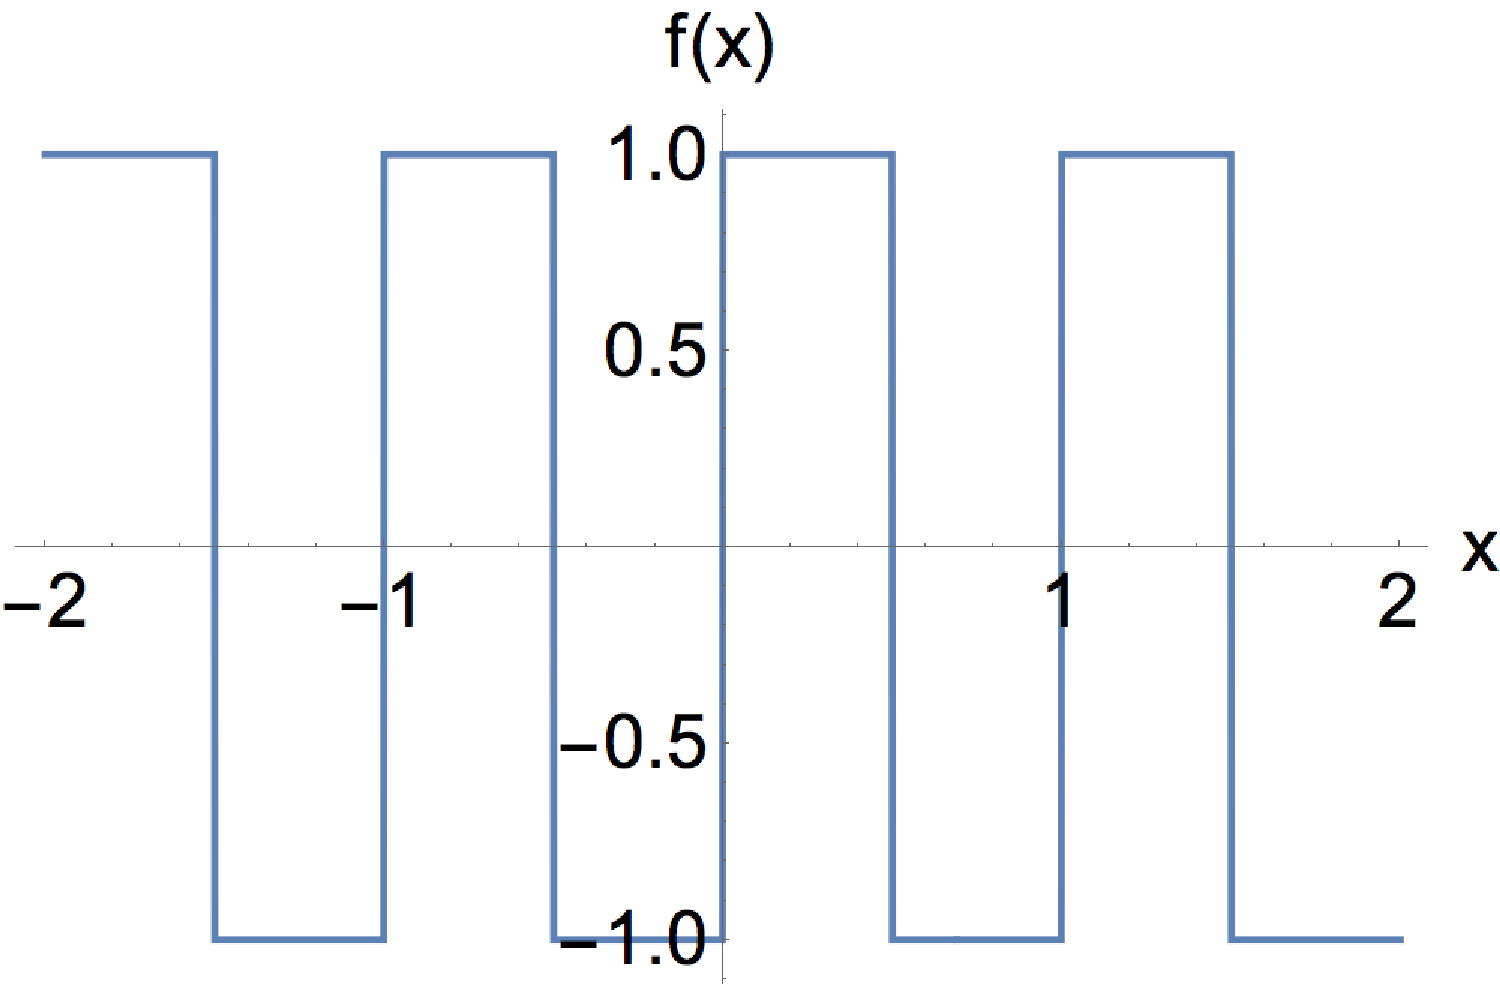
\includegraphics{square_wave.png}

\subsection*{Solution}
\solint{g}{205d04}




%%%%%%%%%%%%%%%%%%%%%%%%%%%%%%%%%
\newpage
%%%%%%%%%%%%%%%%%%%%%%%%%%%%%%%%%

\section{Introduction to sine and cosine Fourier coefficients}
\label{sec:trigcoeff}

\subsection*{Comment}
Fourier series involves the construction of a signal by summing multiple periodic signals and careful choice of each frequency's amplitude and phase. For example, considering the following 3 signals:
\begin{enumerate}
    \item $f_1(t) = 2 \sin(2 \pi t)$
    \item $f_2(t) = 1 \sin(4 \pi t + \pi)$
    \item $f_3(t) = 0.3 \sin(6 \pi t + \pi/5)$
\end{enumerate}
Their sum (k = 1 to 3) produces a much more complex shape:

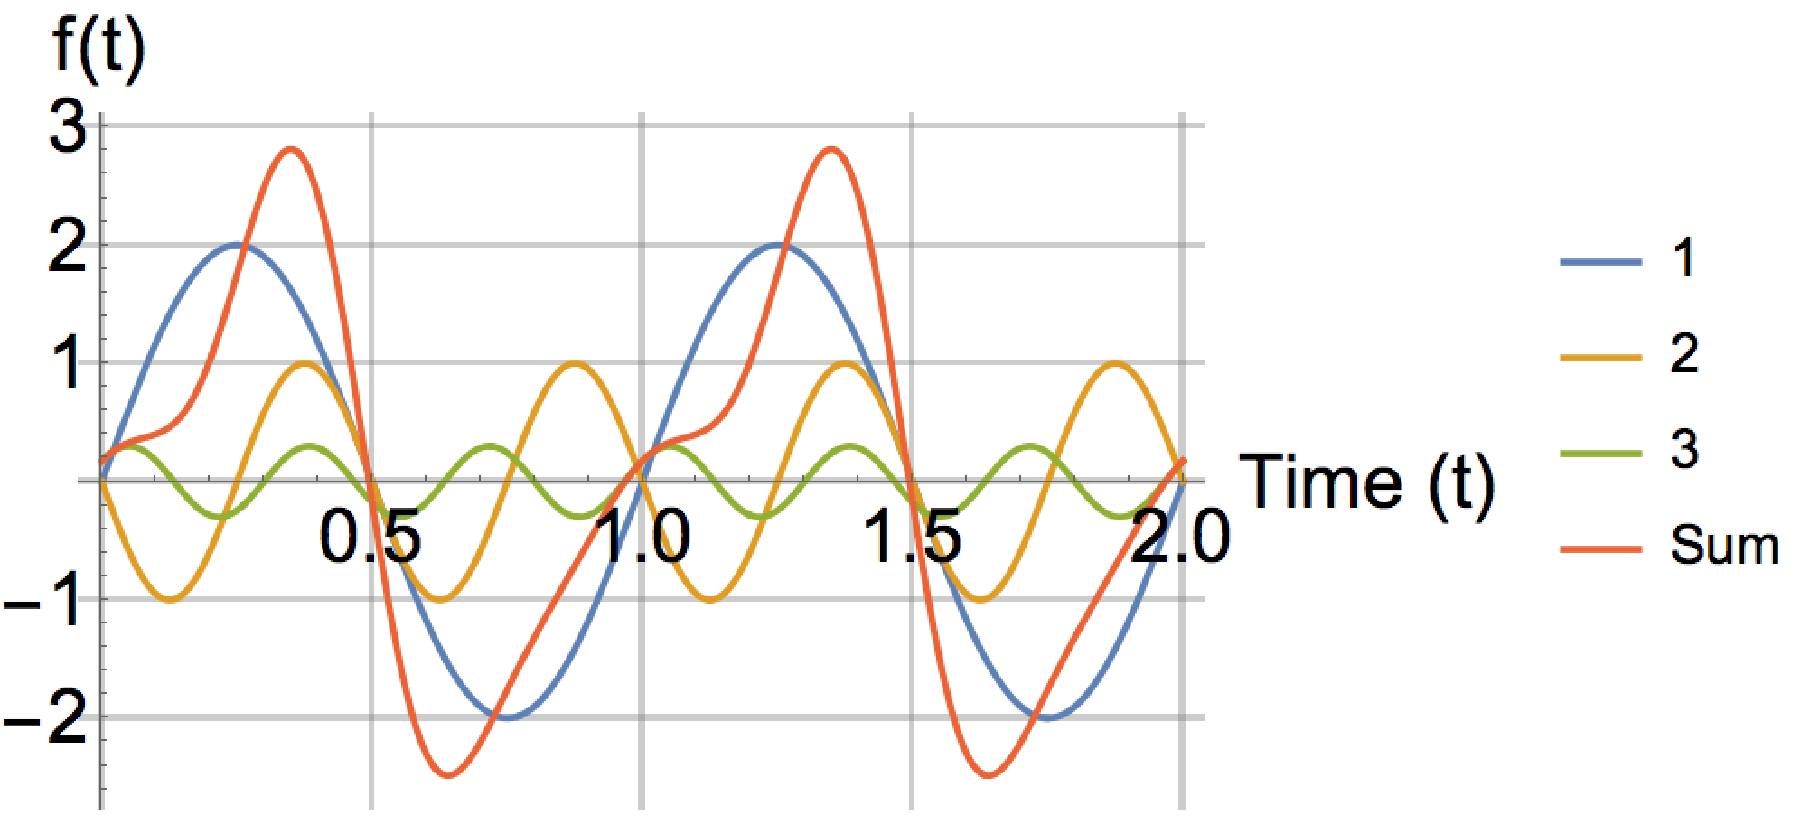
\includegraphics{signal_buildup.png}

Here we will consider Fourier sine and cosine series. We will go beyond this description later, but you should be aware of their existance and a method of their derivation.

\subsection*{Challenge}
As shown above, a complex function (signal) can be made up of a sum of sine signals:
\begin{equation}
    \label{eq:fssinonly}
    f(t) = A_0 + \sum_{k=1}^{N} A_k \sin(2 \pi k t + \phi_k)
\end{equation}

Using basic trigonomatric relations, show that this can be re-written in terms of a sum of sines and cosines:
\begin{equation}
    \label{eq:fssincos}
    f(t) = \frac{a_0}{2} + \sum_{k=1}^{N} a_k \cos(2 \pi k t) + b_k \sin(2 \pi k t)
\end{equation}

I want you to see how the phase information is encoded in the representation of equation \ref{eq:fssincos}. $a_k$ and $b_k$ are referred to as Fourier coefficients. Write an expression for the coefficients $a_k$, $b_k$ and $a_0$.

\subsection*{Solutions}
To check your answer, calculate $a_0$, $a_1$ and $b_1$ given the following information:\\
$A_0=-1/2$, $A_1 = 0.7$, $\phi_1 = \pi/5$.

(make sure your calculator is using radians)

$a_1 = 0.41145$, $b_1 = 0.566312$.

$a_0$:
\soltwodp{f}{75d06e}




%%%%%%%%%%%%%%%%%%%%%%%%%%%%%%%%%
\newpage
%%%%%%%%%%%%%%%%%%%%%%%%%%%%%%%%%

\section{The significance of the Fourier coefficients}

\subsection*{Resources}
\begin{itemize}
    \item Video: \url{https://www.khanacademy.org/science/electrical-engineering/ee-signals/ee-fourier-series/v/ee-fourier-series-intro}
\end{itemize}

\subsection*{Comments}
I recommend to view the suggested resource as this gives a nice introduction to the subject and challenges ahead. Note that the period used in the video is different to that we're using in our description, but you should become comfortable with moving between different notations.

\subsection*{Challenge}
Write a few sentences describing in qualitative terms what the significance of the magnitude of the fourier coefficients $a_k$ and $b_k$ in challenge \ref{sec:trigcoeff} is.

\subsection*{Solutions}
Please compare your answer with your partner or discuss with the teacher in class.



%NT: Students were confused about the interval of integration and how it changes when there is a 2pi inside the brackets or not.
% Add a challenge on getting the appropriate integration limits for different forms of the wave. The key is the modification of the period
% so that one period is complete under different $t$.

%%%%%%%%%%%%%%%%%%%%%%%%%%%%%%%%%
\newpage
%%%%%%%%%%%%%%%%%%%%%%%%%%%%%%%%%
\section{Integral of $\sin(kt)$ and $\cos(kt)$}

\subsection*{Resources}
\begin{itemize}
    \item Video: \url{https://www.khanacademy.org/science/electrical-engineering/ee-signals/ee-fourier-series/v/ee-integral-of-sinmt-and-cosmt}
\end{itemize}

\subsection*{Challenge}
Show that the following integrals evaluate to zero:
\begin{equation}
    \int_0^1 \sin(2 \pi k t) dt = 0
\end{equation}

\begin{equation}
    \int_0^1 \cos(2 \pi k t) dt = 0
\end{equation}

given that $k$ is a non-zero positive integer.

\subsection*{Solutions}
Please compare your answer with your partner or discuss with the teacher in class.




%%%%%%%%%%%%%%%%%%%%%%%%%%%%%%%%%
\newpage
%%%%%%%%%%%%%%%%%%%%%%%%%%%%%%%%%

\section{Integral of product of sines and cosines}

\subsection*{Resources}
\begin{itemize}
    \item Video: \url{https://www.khanacademy.org/science/electrical-engineering/ee-signals/ee-fourier-series/v/ee-integral-sine-times-sine}
    \item Video: \url{https://www.khanacademy.org/science/electrical-engineering/ee-signals/ee-fourier-series/v/ee-integral-cosine-times-cosine}
\end{itemize}

\subsection*{Challenge}
Considering the following integrals, show under what conditions the following integrals evaluate to zero, and what condition they don't evaluate to zero. What is the non-zero evaluation result?

\begin{equation}
    \int_0^1 \sin(2 \pi m t) \sin(2 \pi n t) dt
\end{equation}

\begin{equation}
    \int_0^1 \cos(2 \pi m t) \cos(2 \pi n t) dt
\end{equation}

You may assume that $m$ and $n$ are non-zero positive integers.

\subsection*{Solutions}
Please compare your answer with your partner or discuss with the teacher in class.





%%%%%%%%%%%%%%%%%%%%%%%%%%%%%%%%%
\newpage
%%%%%%%%%%%%%%%%%%%%%%%%%%%%%%%%%
\section{First term in a trigonometric Fourier series}

\subsection*{Resources}
\begin{itemize}
    \item Video: \url{https://www.khanacademy.org/science/electrical-engineering/ee-signals/ee-fourier-series/v/ee-first-term-fourier-series}
\end{itemize}

\subsection*{Challenge}
Considering a fourier series represented by
\begin{equation}
    f(t) = \frac{a_0}{2} + \sum_{k=1}^{N} a_k \cos(2 \pi k t) + b_k \sin(2 \pi k t)
\end{equation}

What is $a_0$ for the following functions?
\begin{enumerate}
    \item $f(t) = \sin(10 \pi t)$
    \item Square wave function $f(t) = \begin{cases} 2 & \text{for } 0<t<1 \\ 1 & \text{for } 1<t<2 \end{cases}$
    \item $f(t) = t^2$ considered only over the interval from $t=0$ to $t=1$
\end{enumerate}

\subsection*{Solutions}
1.\\
\soltwodp{d}{705887}

2.\\
\soltwodp{e}{e1509d}

3.\\
\soltwodp{f}{98680d}




%%%%%%%%%%%%%%%%%%%%%%%%%%%%%%%%%
\newpage
%%%%%%%%%%%%%%%%%%%%%%%%%%%%%%%%%
\section{The Fourier coefficient $a_k$}

\subsection*{Resources}
\begin{itemize}
    \item Video: \url{https://www.khanacademy.org/science/electrical-engineering/ee-signals/ee-fourier-series/v/ee-fourier-coefficients-cosine}
\end{itemize}

\subsection*{Challenge}
Derive an expression for the Fourier coefficient $a_k$ in
\begin{equation}
    f(t) = \frac{a_0}{2} + \sum_{k=1}^{N} a_k \cos(2 \pi k t) + b_k \sin(2 \pi k t)
\end{equation}

Note the difference in period between the above equation and the suggested resource.

\subsection*{Solutions}
Please compare your answer with your partner or discuss with the teacher in class.




%%%%%%%%%%%%%%%%%%%%%%%%%%%%%%%%%
\newpage
%%%%%%%%%%%%%%%%%%%%%%%%%%%%%%%%%
\section{The Fourier coefficient $b_k$}

\subsection*{Resources}
\begin{itemize}
    \item Video: \url{https://www.khanacademy.org/science/electrical-engineering/ee-signals/ee-fourier-series/v/ee-fourier-coefficients-sine}
\end{itemize}

\subsection*{Challenge}
Derive an expression for the Fourier coefficient $b_k$ in
\begin{equation}
    f(t) = \frac{a_0}{2} + \sum_{k=1}^{N} a_k \cos(2 \pi k t) + b_k \sin(2 \pi k t)
\end{equation}

Note the difference in period between the above equation and the suggested resource.

\subsection*{Solutions}
Please compare your answer with your partner or discuss with the teacher in class.




%%%%%%%%%%%%%%%%%%%%%%%%%%%%%%%%%
\newpage
%%%%%%%%%%%%%%%%%%%%%%%%%%%%%%%%%
\section{Trigonometric Fourier series of a square wave}
\label{sec:1stsqwch}

\subsection*{Resources}
\begin{itemize}
    \item Video: \url{https://www.khanacademy.org/science/electrical-engineering/ee-signals/ee-fourier-series/v/ee-fourier-coefficients-for-square-wave}
\end{itemize}

\subsection*{Challenge}
Calculate the Fourier series for the following square-wave:

\begin{equation}
   f(t) =
   \begin{cases}
       1 & \text{for } 0 < t < \frac{1}{2} \\
       0 & \text{for } \frac{1}{2} < t < 1
   \end{cases} 
\end{equation}

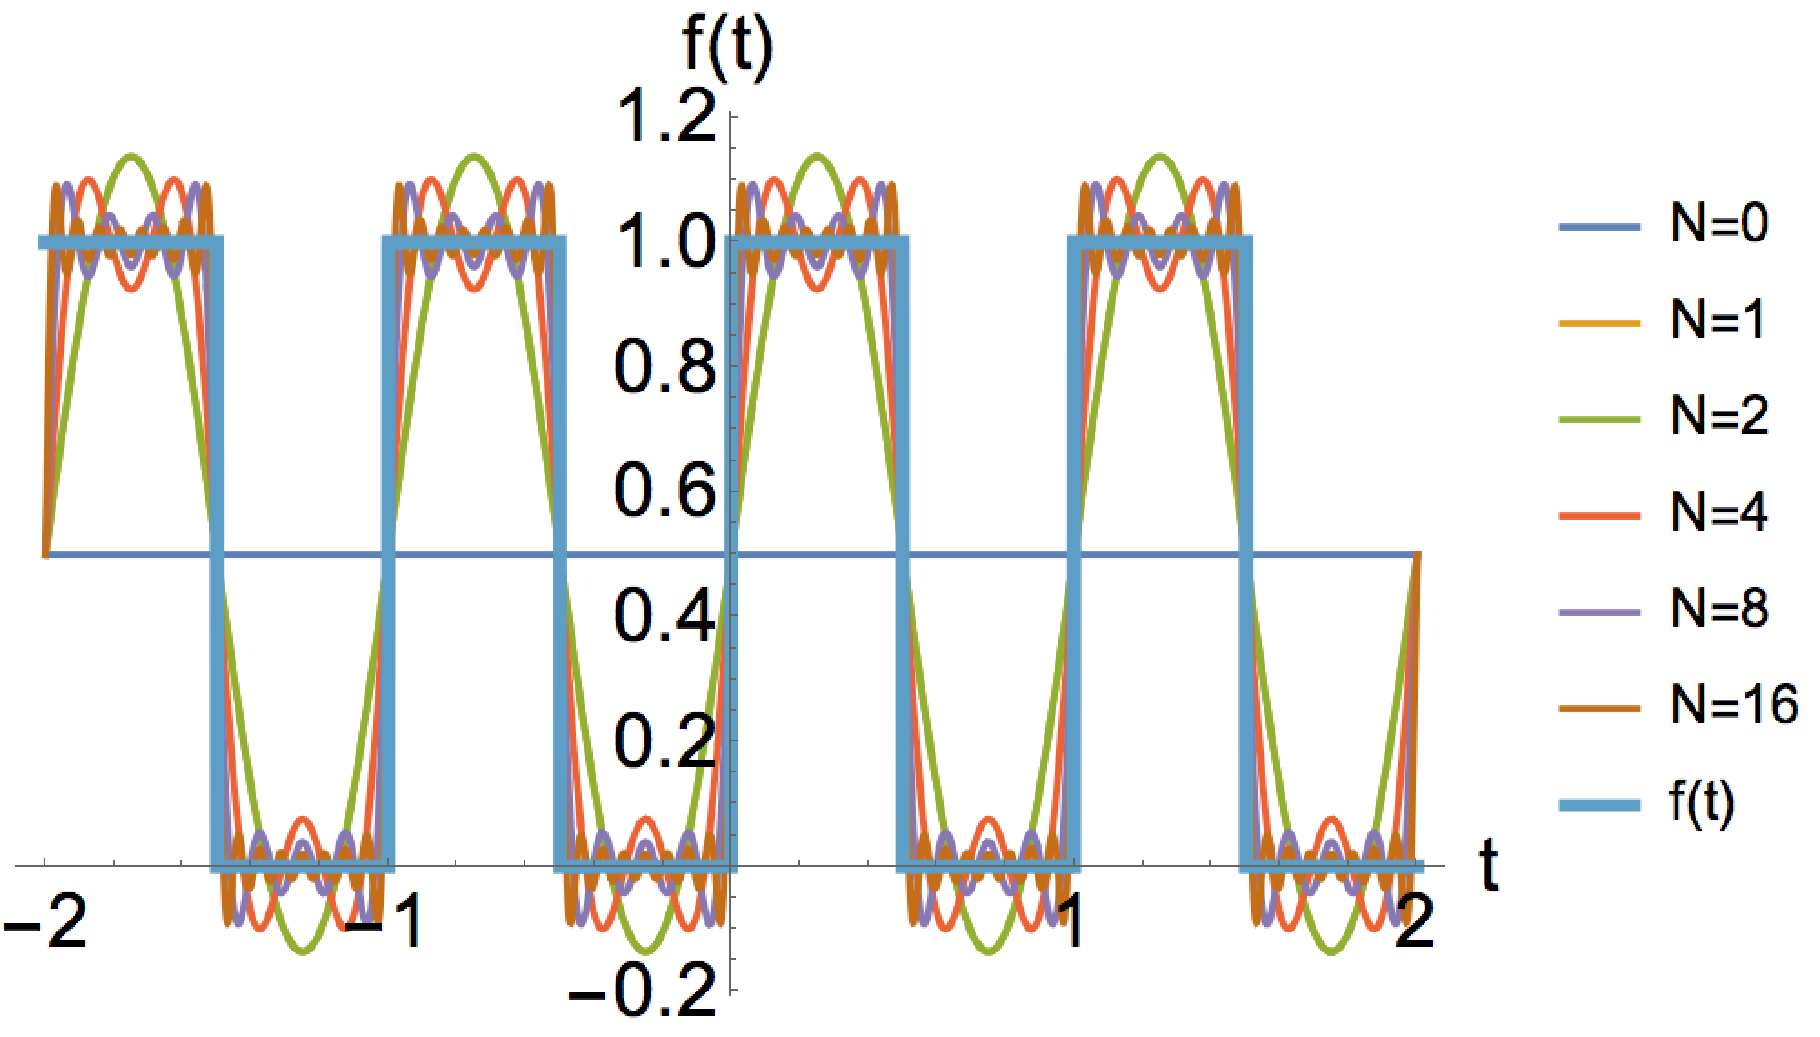
\includegraphics{fourier_sine_series.png}

\subsection*{Solutions}
To check your solution, write out the sum up to $k=2$ and then evaluate $f(0.9)$

0.1258



%%%%%%%%%%%%%%%%%%%%%%%%%%%%%%%%%
\newpage
%%%%%%%%%%%%%%%%%%%%%%%%%%%%%%%%%
\section{Trigonometric Fourier series of another square wave}
\label{sec:2ndsqwch}

\subsection*{Challenge}
Calculate the Fourier series for the following square-wave:

\begin{equation}
   f(t) =
   \begin{cases}
       1 & \text{for } -\frac{1}{4} < t < \frac{1}{4} \\
       0 & \text{for } \frac{1}{4} < t <\frac{3}{4} 
   \end{cases} 
\end{equation}

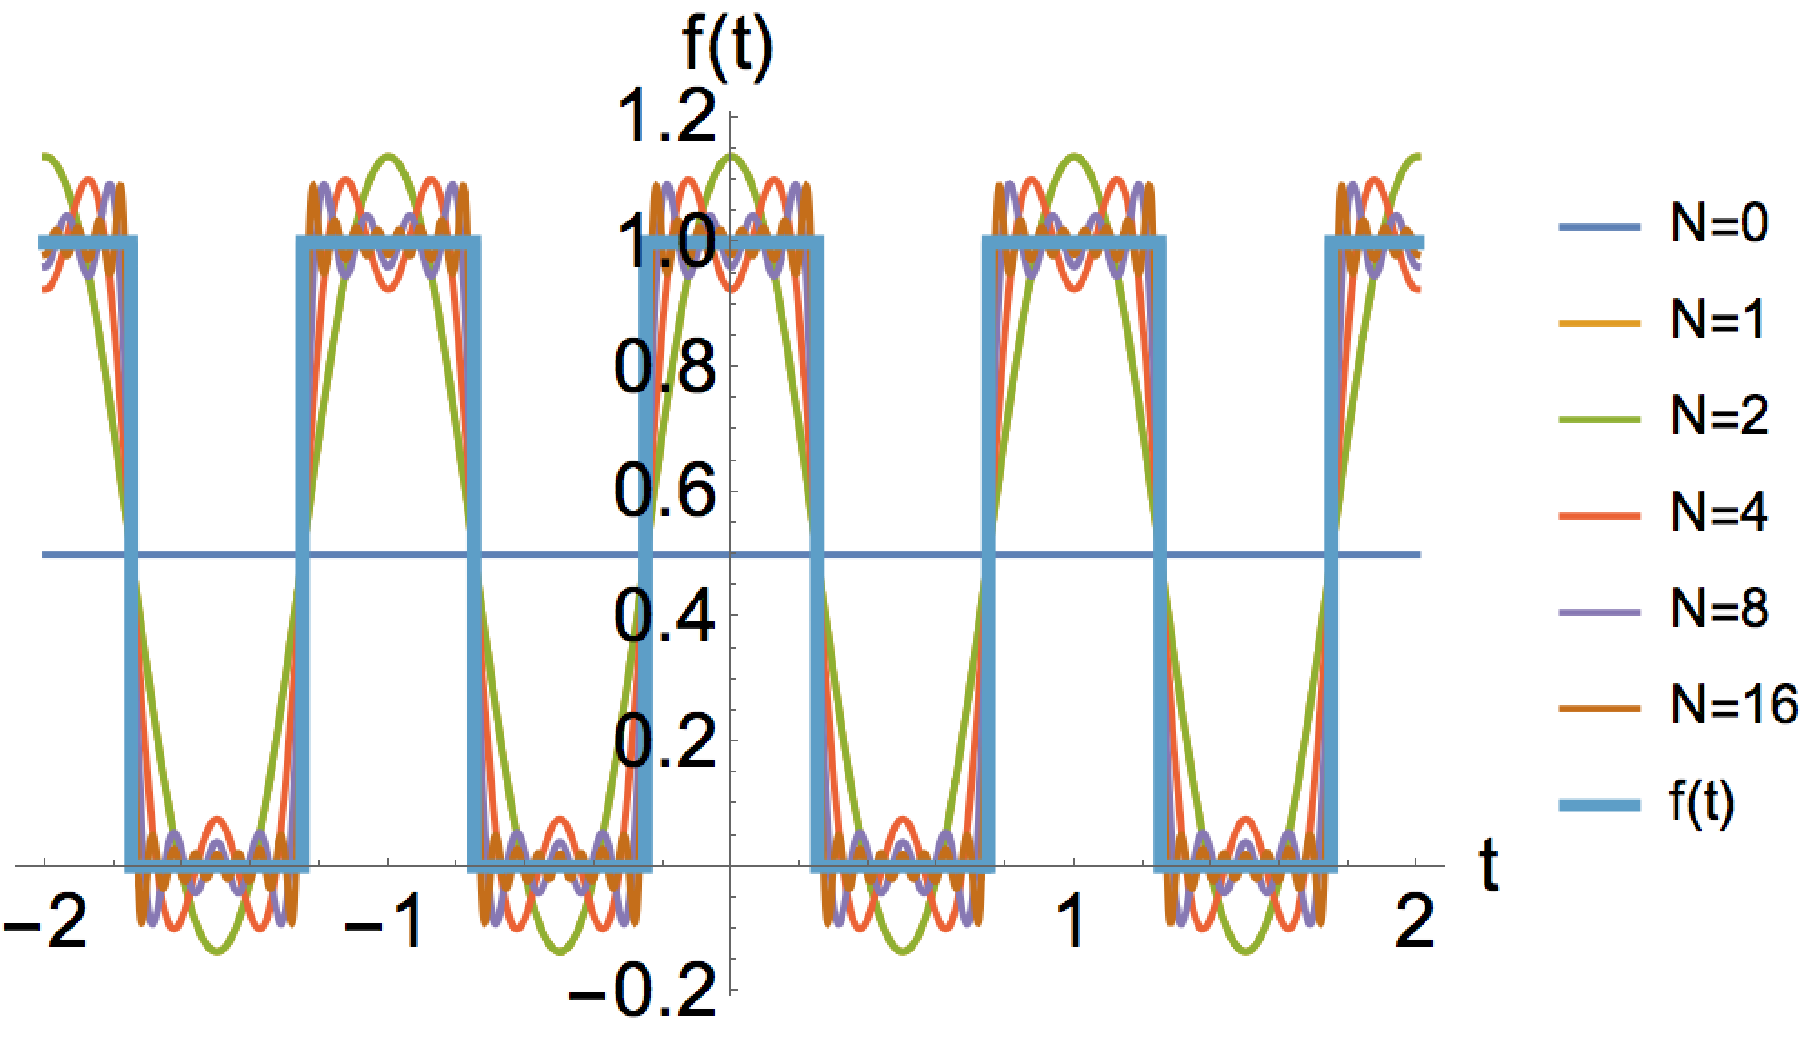
\includegraphics{fourier_cosine_series.png}

\subsection*{Solutions}
To check your solution, write out the sum up to $k=2$ and then evaluate $f(0.7)$

0.30327




%%%%%%%%%%%%%%%%%%%%%%%%%%%%%%%%%
\newpage
%%%%%%%%%%%%%%%%%%%%%%%%%%%%%%%%%
\section{Fourier sine and cosine series}

\subsection*{Challenge}
Considering challenges \ref{sec:1stsqwch} and \ref{sec:2ndsqwch}, one corresponds to a Fourier sine series, and the other to a Fourier cosine series. Such series only contain sine and cosine terms, respectively. (1) State which challenge corresponds to which series, and (2) write a square-wave function that you think would involve both sine and cosine terms.

\subsection*{Solutions}
If you are unsure about your answer, you can either try to solve it to prove it, or please discuss with your partner or ask the teacher.



%%%%%%%%%%%%%%%%%%%%%%%%%%%%%%%%%
\newpage
%%%%%%%%%%%%%%%%%%%%%%%%%%%%%%%%%
\section{Complex numbers}

\subsection*{Resources}
\begin{itemize}
    \item Book: Appendex A starting at page 403 (\url{https://see.stanford.edu/materials/lsoftaee261/book-fall-07.pdf})
\end{itemize}

\subsection*{Challenge}
Considering $z=a+bi$ and $w=c+di$, determine:

1. $z + w$

2. $zw$

3. $z \bar{z}$

4. $z/w$

5. $|z|$

\subsection*{Solutions}
To check your answers, substitute the following values: $a=1$, $b=2$, $c=3$, $d=4$.

1.\\
\solimagint{h}{d8c7d5}

2.\\
\solimagint{i}{3c520b}

3.\\
\solimagint{j}{66248e}

4.\\
\solimagtwodp{k}{39577d}

5.\\
\solimagtwodp{m}{b12a23}




%%%%%%%%%%%%%%%%%%%%%%%%%%%%%%%%%
\newpage
%%%%%%%%%%%%%%%%%%%%%%%%%%%%%%%%%

\section{Complex form of sine and cosine}

\subsection*{Challenge}
Write sine and cosine in terms of complex exponentials.

\subsection*{Solutions}
If you are unsure about your answer, please discuss in class.




%%%%%%%%%%%%%%%%%%%%%%%%%%%%%%%%%
\newpage
%%%%%%%%%%%%%%%%%%%%%%%%%%%%%%%%%
\section{An alternative way to write Fourier series}
\label{sec:expfs}

\subsection*{Comments}
It turns out that a more mathematically-convenient and ultimately intuitive way to write Fourier series is in terms of complex exponentials in the form
\begin{equation}
    \label{eq:fsexp}
    f(t) = \sum_{k=-n}^{k=n} c_k e^{i 2 \pi k t}
\end{equation}

A few things to note:
\begin{itemize}
    \item The sum now runs from $-n$ to $n$.
    \item The $k=0$ term that was originally excluded from the sum in equation \ref{eq:fssincos} is now included.
    \item The $c_k$'s, unlike the $a_k$'s and $b_k$'s, are complex.
    \item $c_{-k} = \bar{c_k}$.
    \item $c_0 = a_0/2$.
\end{itemize}

You see how we started with equation \ref{eq:fssinonly} and now end up with equation \ref{eq:fsexp}? Do you see more-or-less how the phase information is encoded in the $c_k$'s?

\subsection*{Challenge}
1. By comparing equation \ref{eq:fssincos} to equation \ref{eq:fsexp}, write $c_k$ in terms of $a_k$ and $b_k$ for $k<0$ and $k>0$.

2. Show that $c_{-k} = \bar{c_k}$

3. Show that $c_0$ must be $a_0/2$

\subsection*{Solutions}
If you have trouble with the derivation, please discuss in class.




%%%%%%%%%%%%%%%%%%%%%%%%%%%%%%%%%
\newpage
%%%%%%%%%%%%%%%%%%%%%%%%%%%%%%%%%
\section{Integral of a complex exponential over a single period}

\subsection*{Challenge}
Integrate the following function over one period, assuming that $k$ must be an non-zero integer:
\begin{equation}
    g(t) = e^{i 2 \pi k t}
\end{equation}

\subsection*{Solution}
The numerical answer is given below. Be sure you understand why the answer comes out as this number.

\soltwodp{n}{f979e9}




%%%%%%%%%%%%%%%%%%%%%%%%%%%%%%%%%
\newpage
%%%%%%%%%%%%%%%%%%%%%%%%%%%%%%%%%
\section{Derivation of the complex Fourier coefficients}

\subsection*{Resources}
\begin{itemize}
    \item Video starting at 41m 56s: \url{https://www.youtube.com/watch?v=1rqJl7Rs6ps&t=41m56s}
\end{itemize}

\subsection*{Comments}
This is the last major derivation for Fourier series, and parallels what you learned for trigonometric Fourier series. The video does a great job of showing the derivation. Try to become comfortable with manipulating complex exponentials and their periodicity.

\subsection*{Challenge}
Derive an expression for the $c_k$'s in the equation
\begin{equation}
    f(t) = \sum_{k=-n}^{n} c_k e^{i 2 \pi k t} dt
\end{equation}
in terms of the function $f(t)$.

\subsection*{Solution}
Please discuss in class if you are unsure of your derivation.




%%%%%%%%%%%%%%%%%%%%%%%%%%%%%%%%%
\newpage
%%%%%%%%%%%%%%%%%%%%%%%%%%%%%%%%%
\section{Complex Fourier series of a square wave}

\subsection*{Challenge}
1. Determine an expression for the complex Fourier coefficients for the following square wave:
\begin{equation}
   f(t) =
   \begin{cases}
       5 & \text{for } 0 < t < \frac{1}{2} \\
       0 & \text{for } \frac{1}{2} < t < 1
   \end{cases} 
\end{equation}

2. Write the complex Fourier series for the square wave.

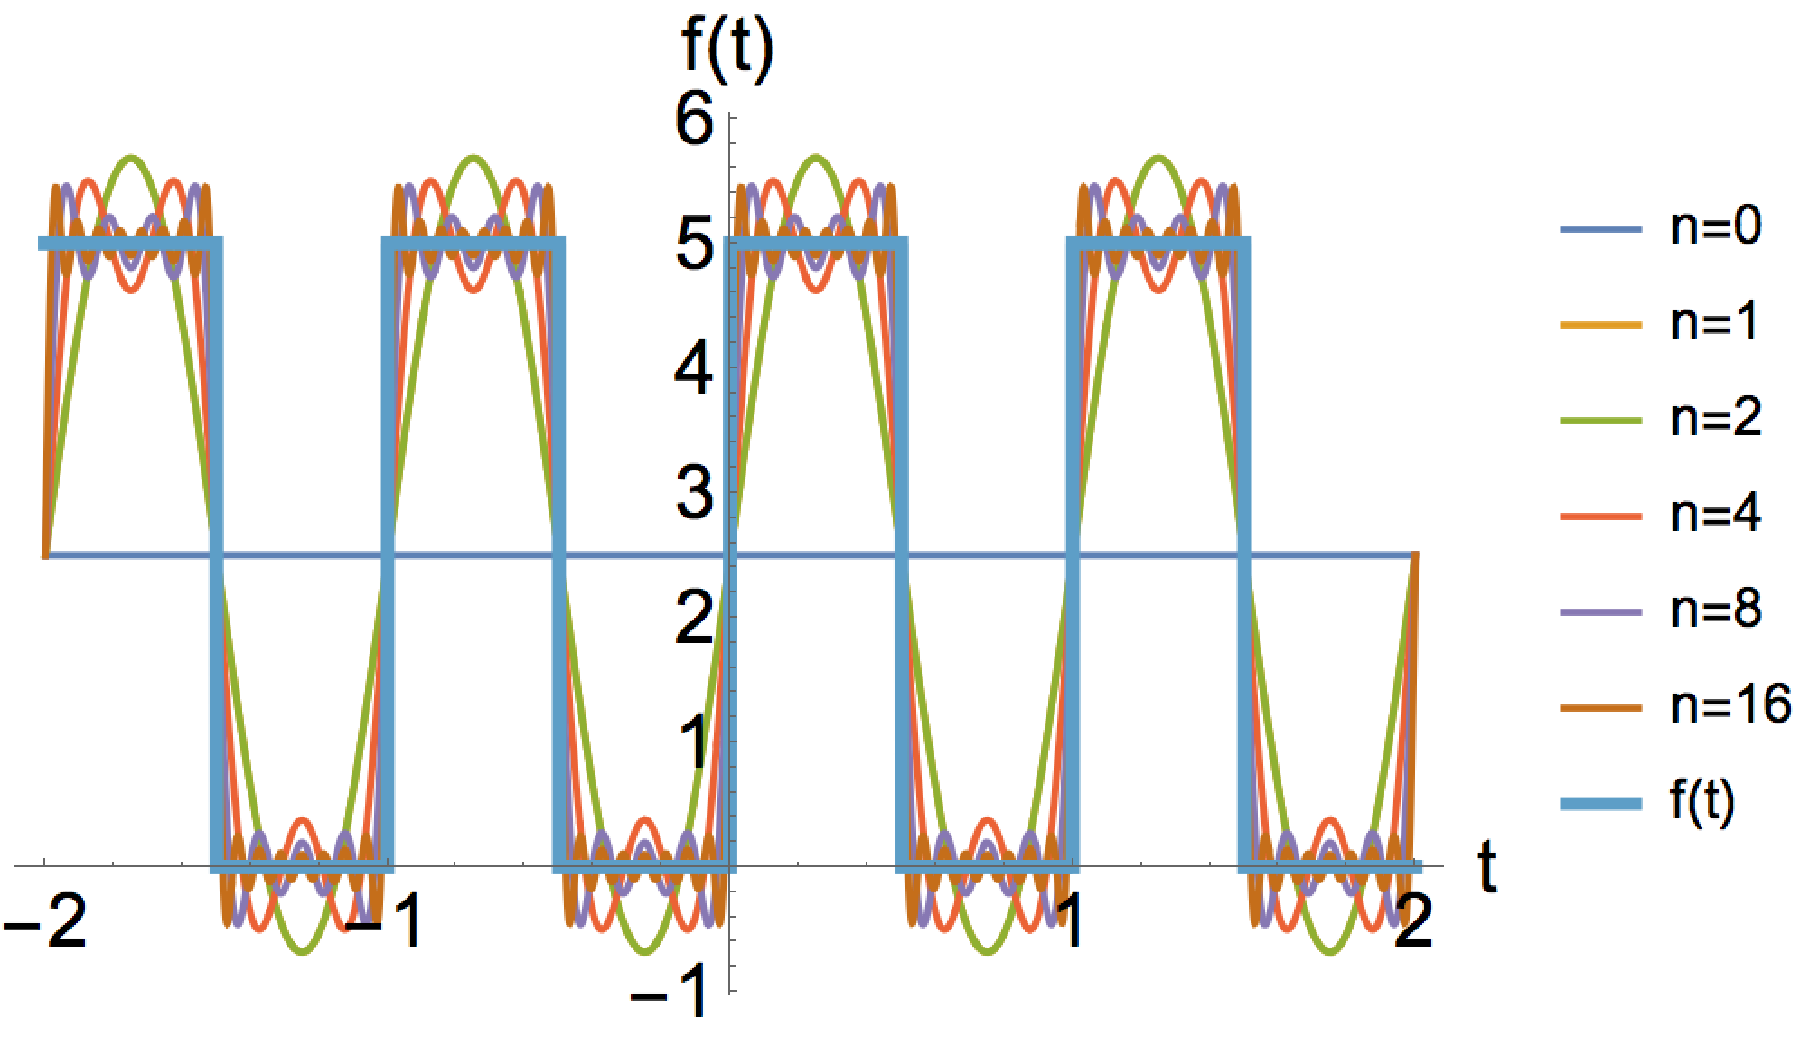
\includegraphics{fs_exp_squarewave.png}

\subsection*{Solution}
1.\\
You should find that $c_{-7} = i 0.227$.

2.\\
If you perform the sum for $n=1$ and evaluate at $t=0.7$, you should obtain a value of $-0.527$.




%%%%%%%%%%%%%%%%%%%%%%%%%%%%%%%%%
\newpage
%%%%%%%%%%%%%%%%%%%%%%%%%%%%%%%%%
\section{Non-unit periods}

\subsection*{Resources}
\begin{itemize}
    \item Book: Chapter 1.6 of the book (\url{https://see.stanford.edu/materials/lsoftaee261/book-fall-07.pdf})
\end{itemize}

\subsection*{Comment}
Until now we considered signals with periodicity 1, but this will not always be the case, and in fact as we make the jump from Fourier series to Fourier transforms this will become more important. The resource gives the intuition behind the non-periodic case for complex Fourier series. For trigonometric Fourier series, the Fourier coefficients become:
\begin{equation}
    a_k = \frac{2}{T} \int_{t_0}^{t_0+T} f(t) \cos(2 \pi k t/T) dt
\end{equation}
\begin{equation}
    b_k = \frac{2}{T} \int_{t_0}^{t_0+T} f(t) \sin(2 \pi k t/T) dt
\end{equation}

while for complex Fourier series the Fourier coefficients become:
\begin{equation}
    c_k = \frac{1}{T} \int_{t_0}^{t_0+T} f(t) e^{-i 2 \pi kt/T} dt
\end{equation}

\subsection*{Challenge}
Obtain an expression for the exponential Fourier series for the pulsing sawtooth function
\begin{equation}
    f(t)=
    \begin{cases}
        t & \text{for } 0<t<\frac{1}{4} \\
        0 & \text{for } \frac{1}{4}<t<\frac{1}{2}
    \end{cases}
\end{equation}

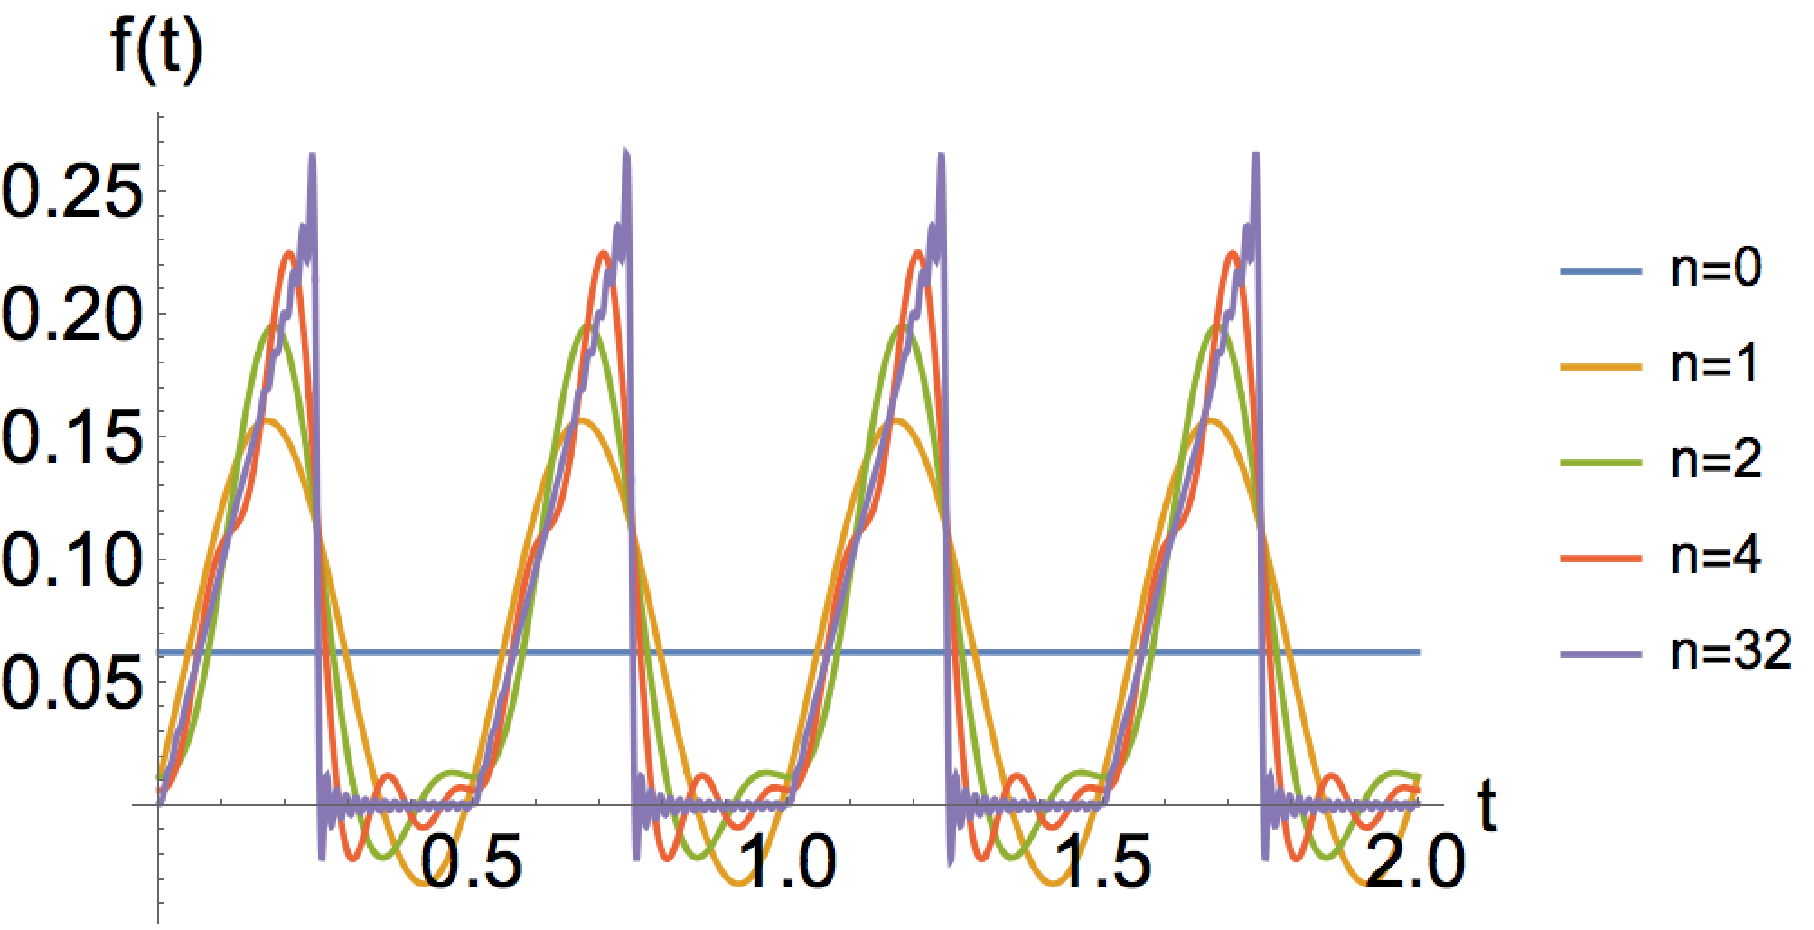
\includegraphics[scale=0.7]{sawwave.png}

\subsection*{Solution}
You should find the $c_k$'s for $k \ne 0$ are
\begin{equation}
    \frac{i \pi k e^{-i \pi k} + e^{-i \pi k} - 1}{8 \pi^2 k^2}
\end{equation}



%%%%%%%%%%%%%%%%%%%%%%%%%%%%%%%%%
\newpage
%%%%%%%%%%%%%%%%%%%%%%%%%%%%%%%%%
\section{Gibb's phenomenon}

\subsection*{Resources}
\begin{itemize}
    \item Book: 1.18 (\url{https://see.stanford.edu/materials/lsoftaee261/book-fall-07.pdf})
\end{itemize}

\subsection*{Challenge}
1. Qualitatively speaking, what is the Gibb's phenomenon?

2. Considering a square wave of the form
\begin{equation}
    f(t)=
    \begin{cases}
        -1 & \text{for } -\frac{1}{2} < t < 0 \\
        1 & \text{for } 0 < t < \frac{1}{2}
    \end{cases}
\end{equation}
as the sum of the Fourier series goes to infinity, what is the maximum value of the signal?

\emph{The full derivation is beyond the scope of this course, so it is not necessary to understand the derivation in the notes. The aim of this challenge is simply to enable you to be able to describe qualitatively what Gibb's phenomenon is using a few sentences, and know the amount of overshoot in the case of a standard $\pm 1$ square-wave.}

\subsection*{Solution}
2.\\
\soltwodp{m}{d9c018}




%%%%%%%%%%%%%%%%%%%%%%%%%%%%%%%%%
\newpage
%%%%%%%%%%%%%%%%%%%%%%%%%%%%%%%%%
\section{Fourier coefficients of sin(x)}
\label{sec:fcsinx}

\subsection*{Challenge}
By writing $\sin(x)$ in exponential form, deduce the Fourier coefficients $c_{-2}$, $c_{-1}$ and $c_0$. Try to do this by inspection rather than application of formulas.

\subsection*{Solutions}
$c_{-2}$:\\
\solimagtwodp{h}{53126e}

$c_{-1}$:\\
\solimagtwodp{k}{312a1a}

$c_0$:\\
\solimagtwodp{j}{b6ffa8}




%%%%%%%%%%%%%%%%%%%%%%%%%%%%%%%%%
\newpage
%%%%%%%%%%%%%%%%%%%%%%%%%%%%%%%%%

\section{Fourier Coefficients of 1 + sin(x)}
\label{sec:fcsinxp1}

\subsection*{Challenge}
Using the same approach as challenge \ref{sec:fcsinx}, deduce for the function $1+sin(x)$ the Fourier coefficients $c_{-1}$, $c_0$ and $c_1$.

\subsection*{Solutions}
$c_{-1}$:\\
\solimagtwodp{m}{434572}

$c_0$:\\
\solimagtwodp{n}{1444ea}

$c_1$:\\
\solimagtwodp{o}{2e5a62}





%%%%%%%%%%%%%%%%%%%%%%%%%%%%%%%%%
\newpage
%%%%%%%%%%%%%%%%%%%%%%%%%%%%%%%%%

\section{Relation of positive and negative Fourier coefficients for a real signal}

\subsection*{Resources}
\begin{itemize}
    \item Challenge \ref{sec:expfs}
    \item Book: 1.4 (\url{https://see.stanford.edu/materials/lsoftaee261/book-fall-07.pdf})
    \item Video: Lecture 2 (\url{https://www.youtube.com/watch?v=1rqJl7Rs6ps})
\end{itemize}

\subsection*{Challenge}
If the Fourier coefficient $C_1$ is $4 + 6i$ for a real signal, what is the Fourier coefficient $C_{-1}$?

\subsection*{Solution}
\solimagint{p}{de57ee}




%%%%%%%%%%%%%%%%%%%%%%%%%%%%%%%%%
\newpage
%%%%%%%%%%%%%%%%%%%%%%%%%%%%%%%%%
\section{2D orthogonal vectors}

\subsection*{Resources}
\begin{itemize}
    \item Book: 1.9 (\url{https://see.stanford.edu/materials/lsoftaee261/book-fall-07.pdf})
\end{itemize}

\subsection*{Challenge}
Sum the points of the vectors in 2D that are orthogonal:

1 point: (5, 4) and (-1, 1.25)

2 points:  (2, -3) and (-6, 4)

4 points: (-2.25, 1.5) and (2, 3)

8 points: (4.5, 4) and (3, -3.375)

16 points: (6, 4) and (4, -6)

32 points: (5, 1) and (-2, 8.125)

64 points: (0, 1) and (1, 0)

128 points: (1, 1) and (1, 1)

\subsection*{Solution}
\solint{q}{919325}




%%%%%%%%%%%%%%%%%%%%%%%%%%%%%%%%%
\newpage
%%%%%%%%%%%%%%%%%%%%%%%%%%%%%%%%%
\section{Orthonormal basis}

\subsection*{Resources}
\begin{itemize}
    \item Video: \url{https://www.khanacademy.org/math/linear-algebra/alternate-bases/orthonormal-basis/v/linear-algebra-introduction-to-orthonormal-bases}
\end{itemize}

\subsection*{Challenge}
Sum the points of the following vectors that form an orthonormal basis:

1 point :
($\displaystyle \frac{1}{\sqrt{5}}, \frac{2}{\sqrt{5}}$) and
($\displaystyle \frac{2}{\sqrt{5}}, \frac{4}{\sqrt{5}}$)

2 points:
($\displaystyle \frac{2}{\sqrt{5}}$, $\displaystyle \frac{1}{\sqrt{5}}$) and
($\displaystyle \frac{-1}{\sqrt{5}}$, $\displaystyle \frac{2}{\sqrt{5}}$)

4 points:
($\displaystyle \frac{2}{\sqrt{2}}, \sqrt{\frac{7}{8}}, \frac{1}{\sqrt{6}}$),
($\displaystyle -\sqrt{\frac{2}{5}}, \frac{7}{\sqrt{14}}, -\frac{1}{\sqrt{6}}$) and
($\displaystyle \frac{1}{\sqrt{3}},  \frac{1}{5 \sqrt{3}}, -\frac{7}{5 \sqrt{3}}$)

8 points:
($\displaystyle \frac{1}{\sqrt{21}}, \frac{2}{\sqrt{21}}, \frac{4}{\sqrt{21}}$),
($\displaystyle -\sqrt{\frac{2}{7}}, \frac{3}{\sqrt{14}}, -\frac{1}{\sqrt{14}}$) and
($\displaystyle \sqrt{\frac{2}{3}},  \frac{1}{\sqrt{6}}, -\frac{1}{\sqrt{6}}$)

%16 points:
%($\displaystyle \frac{1}{\sqrt{6}}, \sqrt{\frac{2}{3}}, \frac{1}{\sqrt{6}}$),
%($\displaystyle -\frac{1}{\sqrt{2}},  \frac{2 \sqrt{2}}{5}, -\frac{3}{5 \sqrt{2}}$) and
%($\displaystyle \frac{1}{\sqrt{3}},  \frac{1}{5 \sqrt{3}}, -\frac{7}{5 \sqrt{3}}$)

16 points:
($0, 2$) and ($2, 0$)

32 points:
($0, 1$) and ($1, 0$)

\subsection*{Solution}
\solint{r}{3b1939}




%%%%%%%%%%%%%%%%%%%%%%%%%%%%%%%%%
\newpage
%%%%%%%%%%%%%%%%%%%%%%%%%%%%%%%%%
\section{Natural basis}

\subsection*{Resources}
\begin{itemize}
    \item Book: 1.9 (\url{https://see.stanford.edu/materials/lsoftaee261/book-fall-07.pdf})
\end{itemize}

\subsection*{Challenge}
Sum the components of the following vectors of a natural basis in $\mathbb{R}^{300}$ space:

\begin{itemize}
    \item First component of the first vector
    \item first component of the second vector
    \item 200th component of the 100th vector
    \item 200th component of the 200th vector
    \item last component of the 299th vector
    \item last component of the last vector
\end{itemize}

\subsection*{Solution}
\solint{s}{c0828e}




%%%%%%%%%%%%%%%%%%%%%%%%%%%%%%%%%
\newpage
%%%%%%%%%%%%%%%%%%%%%%%%%%%%%%%%%
\section{Orthonormal basis for Fourier series}

\subsection*{Resources}
\begin{itemize}
    \item Book: 1.9 (\url{https://see.stanford.edu/materials/lsoftaee261/book-fall-07.pdf})
    \item Video: Lecture 4 (\url{https://www.youtube.com/watch?v=n5lBM7nn2eA})
\end{itemize}

\subsection*{Comment}
The previous challenges have focussed on the orthogonality and orthonormality of vectors. We now make the jump to functions. As chapter 1.9 explains, although its not perfect, the analogy between vectors and functions is a good way to help understand and visualise the role that the terms of a Fourier series play in defining a basis upon which to describe a function.

\subsection*{Challenge}
By evaluating the following functions, show that the terms of a Fourier series form an orthonormal basis:

$y_1(t) = (e^{2 \pi i k_1 t}, e^{2 \pi i k_1 t})$

$y_2(t) = (e^{2 \pi i k_1 t}, e^{2 \pi i k_2 t})$

\subsection*{Solution}
$y_1(t)$:\\
\solint{x}{6dbf9a}

$y_2(t)$:\\
\solint{y}{f05e43}




%%%%%%%%%%%%%%%%%%%%%%%%%%%%%%%%%
\newpage
%%%%%%%%%%%%%%%%%%%%%%%%%%%%%%%%%
\section{Circles and Fourier series}

\subsection*{Resources}
\begin{itemize}
    \item Video 1: \url{https://www.youtube.com/watch?v=Y9pYHDSxc7g}
    \item Video 2: \url{https://www.youtube.com/watch?v=LznjC4Lo7lE}
\end{itemize}

\subsection*{Comment}
In the first lecture we saw how it was possible to approximate any function given enough circles. Here we link what you have learned back to that first lecture. I strongly recommend viewing the fun and informative videos listed here under Resources. In summary, by building a Fourier series you are representing a function using an orthonormal basis, where each component of the basis can be considered visually as a circle operating with individual radius and frequency on the real-imaginary plane.

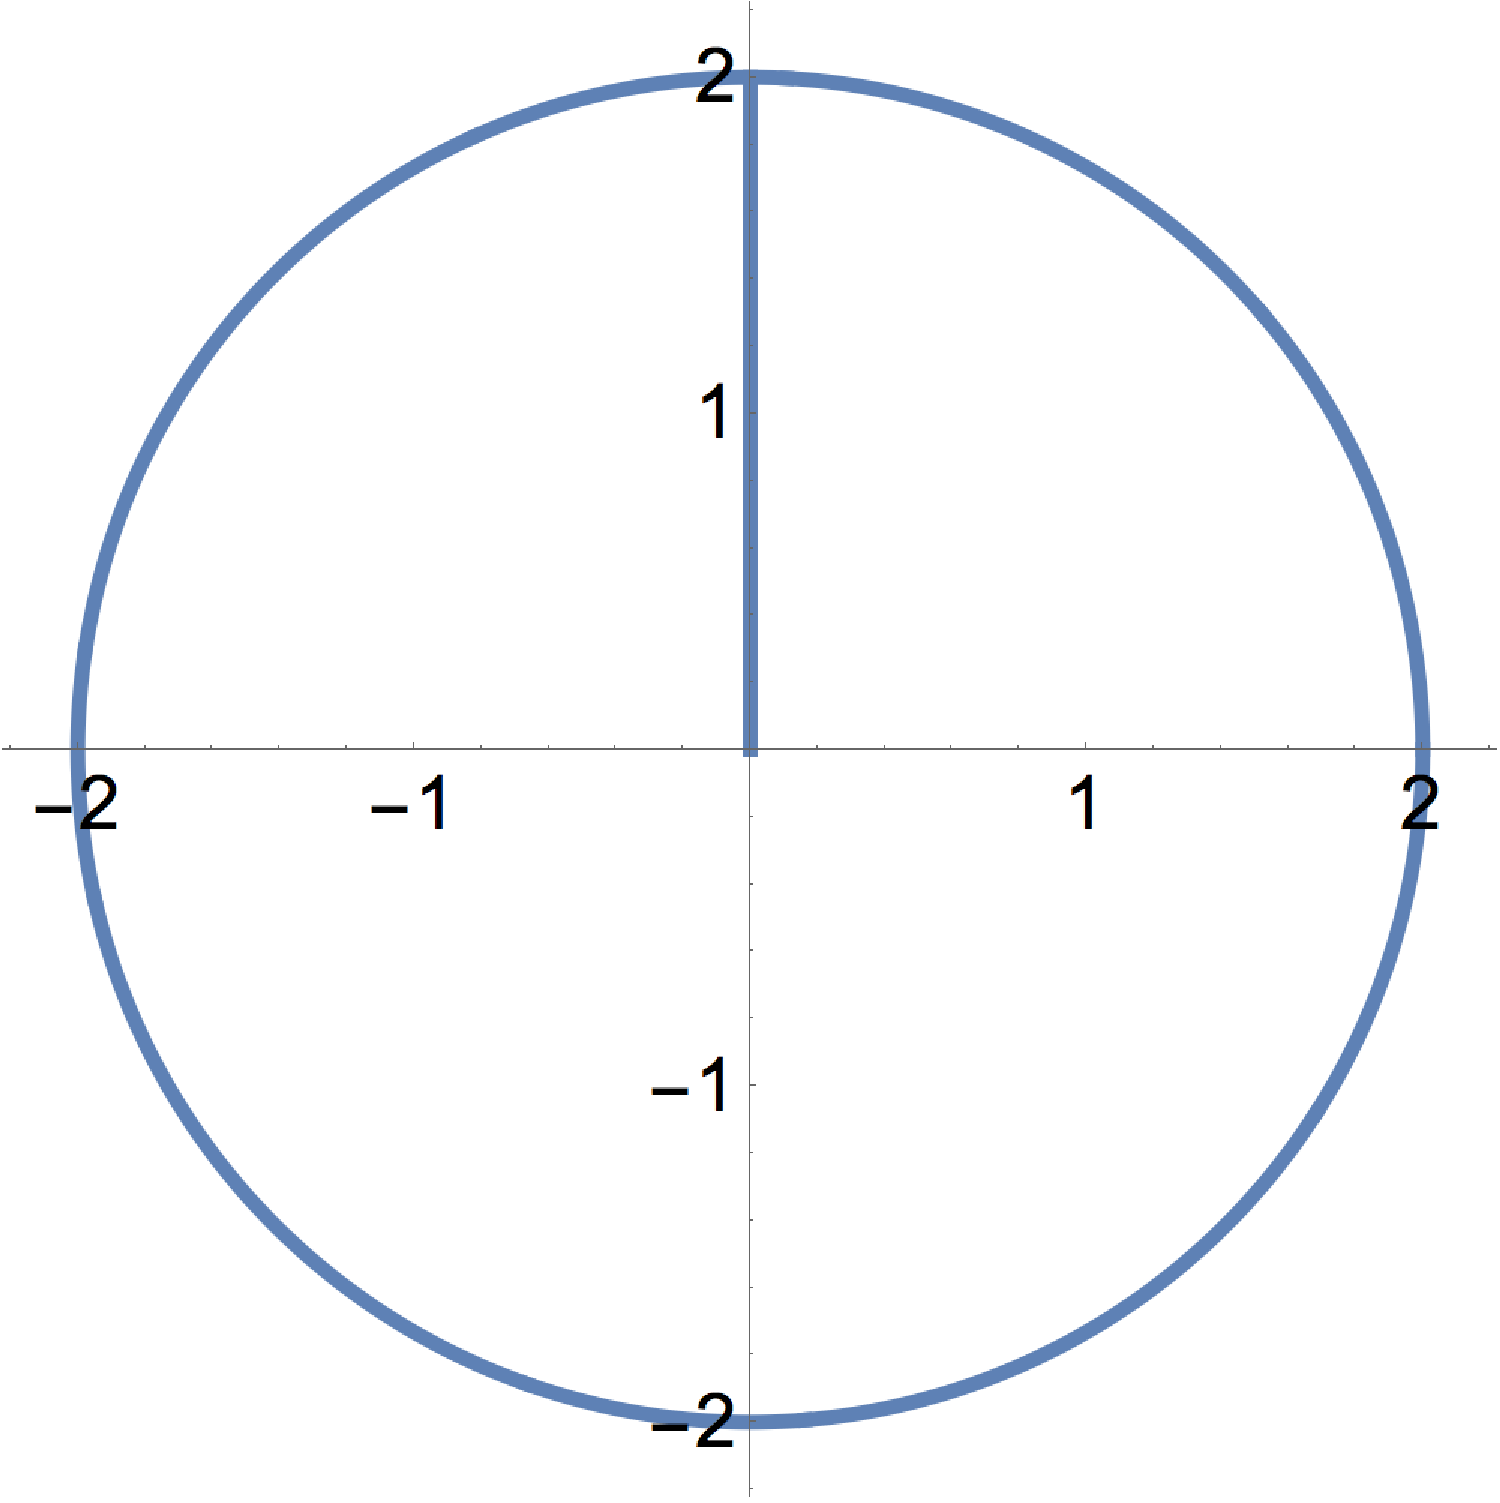
\includegraphics[scale=0.5]{circle.png}

\subsection*{Challenge}
Treating the x-axis as the real axis and the y-axis as the imaginary axis, arrange the equations below in the following order:

\begin{enumerate}
    \item A point moving round on a circle with radius 2 units and frequency 2 Hz
    \item A point moving round on a circle with radius 3 units and frequency 1 Hz
    \item A point moving round on a circle with radius 2 units and a period of 1 second
    \item A point moving round on a circle with radius 3 units and a period of 2 seconds
\end{enumerate}

Equations:

$\displaystyle A e^{2 \pi i k t}$ where $t$ is time in seconds and the values of $A$ and $k$ are as follows:

A: $A=2$, $k=2$ 

B: $A=3$, $k=1$

C: $A=3$, $k=0.5$

D: $A=2$, $k=1$

\subsection*{Solution}
\solstr{t}{d8a7e6}




\iffalse
%%%%%%%%%%%%%%%%%%%%%%%%%%%%%%%%%
\newpage
%%%%%%%%%%%%%%%%%%%%%%%%%%%%%%%%%
\section{Partial derivatives}

\subsection*{Challenge}
Determine $u_t$ and $u_{xx}$ for the equation

\begin{equation}
    u(x,t) = 5tx^2 + 3t - x
\end{equation}

To check your answer, substitute $x=3$ and $t=2$ into your answers, as appropriate.

\subsection*{Solution}
$u_t$:\\
\solint{t}{4fb068}

$u_{xx}$:\\
\solint{x}{53502b}




%%%%%%%%%%%%%%%%%%%%%%%%%%%%%%%%%
\newpage
%%%%%%%%%%%%%%%%%%%%%%%%%%%%%%%%%
\section{Heat equation: Periodicity}

\subsection*{Resources}
\begin{itemize}
    \item Book: Section 1.13.1 (\url{https://see.stanford.edu/materials/lsoftaee261/book-fall-07.pdf})
    \item Lecture 4 from 37:00 onwards: (\url{https://www.youtube.com/watch?v=n5lBM7nn2eA}), continuing at the start of lecture 5 (\url{https://www.youtube.com/watch?v=X5qRpgfQld4})
\end{itemize}

\subsection*{Comment}
Here we can learn about an application of Fourier series to solve partial differential equations. This problem was one of the motivations for Fourier to develop the idea of Fourier series.

The motivation for the equation $u_t = \frac{1}{2} u_{xx}$ described in the notes is complicated somewhat by the interpretation in terms of equivalences between electrical and thermal capacitance. If this is not so clear then don't worry about it. At a minimum you should understand the following:
\begin{itemize}
    \item Heat flow is proportional to the gradient of the temperature.
    \item Heat accumulates within a unit volume when the rate of heat flow into that volume is greater than the rate of heat flow out of that volume.
\end{itemize}

\subsection*{Challenge}
The following statements concern a heated ring with circumference 1 and temperature distribution described by $u(x,t)$. Add the points of the statements that are defined by the system to be true:

1 point: $\displaystyle u(x,t) = u(x,t)$

2 points: $\displaystyle u(x,t) = u(x,t+1)$

4 points: $\displaystyle u(x,t) = u(x,t+2)$

8 points: $\displaystyle u(x,t) = u(x+1,t)$

16 points: $\displaystyle u(x,t) = u(x+1,t+1)$

32 points: $\displaystyle u(x,t) = u(x+1,t+2)$

64 points: $\displaystyle u(x,t) = u(x+2,t)$

128 points: $\displaystyle u(x,t) = u(x+2,t+1)$

256 points: $\displaystyle u(x,t) = u(x+2,t+2)$

512 points: The temperature distribution is periodic in space but not time

1024 points: The temperature distribution is periodic in time but not space

2048 points: The temperature distribution is periodic in both space and time

4096 points: The temperature distribution is periodic neither in space nor time


\subsection*{Solution}
\solint{y}{2259d1}




%%%%%%%%%%%%%%%%%%%%%%%%%%%%%%%%%
\newpage
%%%%%%%%%%%%%%%%%%%%%%%%%%%%%%%%%
\section{Heat equation on a ring: derivation}
\label{sec:heateqnfc}

\subsection*{Resources}
\begin{itemize}
    \item Video: \url{https://www.youtube.com/watch?v=yAOCibHPgLA}
    \item Book: Section 1.13.1 (\url{https://see.stanford.edu/materials/lsoftaee261/book-fall-07.pdf})
    \item Lecture 4 from 37:00 onwards: (\url{https://www.youtube.com/watch?v=n5lBM7nn2eA}), continuing at the start of lecture 5 (\url{https://www.youtube.com/watch?v=X5qRpgfQld4})
\end{itemize}

\subsection*{Challenge}
Starting from the heat (diffusion) equation $u_t = u_{xx}/2$, show that the general solution to the heat equation on a ring is given by
\begin{equation}
    u(x,t) = \sum_{n=-\infty}^{n=\infty} c_n(0) e^{-2 \pi^2 n^2 t} e^{i 2 \pi n x}
\end{equation}
and write an expression for $c_n(0)$ in terms of the initial temperature distribution $u(x,0)$.

\subsection*{Solution}
Please compare with your peers during discussion time and ask if there is anything you do not understand.




%%%%%%%%%%%%%%%%%%%%%%%%%%%%%%%%%
\newpage
%%%%%%%%%%%%%%%%%%%%%%%%%%%%%%%%%
\section{Heat equation on a ring: calculation}
\label{sec:heateqn}

\subsection*{Comment}
Remember that any integer multiple of $2 \pi$ in the complex exponential (eg, $e^{i 4 \pi}$ or $e^{i 2 \pi n}$ where $n$ is an integer) is equivalent to having $2 \pi$ in the exponential due to the periodic nature of complex exponentials (ie, that $e^{i 2 \pi} = \cos(2 \pi) + i \sin(2 \pi)$ and $\cos(2 \pi) = \cos(4 \pi) = \cos(6 \pi)$ etc).

\subsection*{Challenge}
Consider an initial heat distribution around a ring. Relative to ambient temperature, the initial temperature distribution follows a cosine distribution with the peak temperature at $x=0$.

1. Write an expression for the initial relative temperature distribution, $u(x,0)$, assuming the ring has a circumference of 1 unit.

2. Determine $c_{n=\pm 1}(0)$ and $c_{n \ne 1}(0)$

3. Write an expression for the temperature distribution as a function of position and time $u(x,t)$.

You can see an animation of the solution here:\\
\url{https://raw.githubusercontent.com/NanoScaleDesign/FourierAnalysis/master/Images/cosrelax.gif}

\subsection*{Solution}
1. You should find that your temperature distribution satisfies the result:\\
$u(0.2,0) = 0.309$

2.\\
$c_{n=\pm 1}(0)$\\
\soltwodp{b}{06ac46}

$c_{n \ne 1}(0)$\\
\soltwodp{a}{690969}

3. To check your answer you may substitute $x=0.3$ and $t=0.01$ into your solution:\\
$u(0.3,0.01) = -0.25$

\fi

% Convergence?
